%==============================================================================
% Figure: Fractal Large-Scale Structure
% Chapter: 13 - Origami Dimensions
% Data: fractal_lss.json
%==============================================================================
% Purpose: Visualize Genesis prediction of fractal galaxy distribution with
%          Hausdorff dimension d_f = 2.2-2.4 via N(r) ~ r^{d_f} scaling.
%          Shows departure from homogeneous d_f = 3 distribution.
%==============================================================================

\begin{figure}[htbp]
  \centering

  % Cumulative galaxy counts N(r) vs r (log-log plot)
  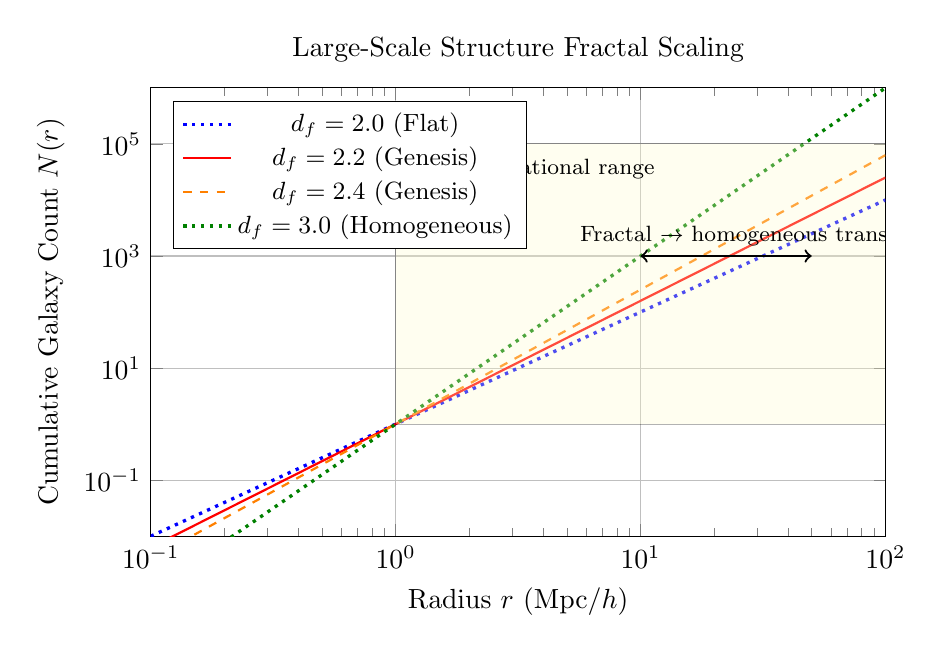
\begin{tikzpicture}
    \begin{loglogaxis}[
      width=0.9\textwidth,
      height=0.6\textwidth,
      title={Large-Scale Structure Fractal Scaling},
      xlabel={Radius $r$ (Mpc/$h$)},
      ylabel={Cumulative Galaxy Count $N(r)$},
      xmin=0.1, xmax=100,
      ymin=0.01, ymax=1e6,
      grid=major,
      legend pos=north west,
      legend style={font=\small},
    ]
    % Flat 2D (d_f = 2.0)
    \addplot[
      blue, dotted, very thick,
      domain=0.1:100,
      samples=50,
    ] {x^2};
    \addlegendentry{$d_f = 2.0$ (Flat)}

    % Genesis prediction d_f = 2.2
    \addplot[
      red, thick,
      domain=0.1:100,
      samples=50,
    ] {x^2.2};
    \addlegendentry{$d_f = 2.2$ (Genesis)}

    % Genesis prediction d_f = 2.4
    \addplot[
      orange, thick, dashed,
      domain=0.1:100,
      samples=50,
    ] {x^2.4};
    \addlegendentry{$d_f = 2.4$ (Genesis)}

    % Homogeneous 3D (d_f = 3.0)
    \addplot[
      green!50!black, dotted, very thick,
      domain=0.1:100,
      samples=50,
    ] {x^3};
    \addlegendentry{$d_f = 3.0$ (Homogeneous)}

    % Observational range annotation
    \draw[fill=yellow!20, opacity=0.3] (axis cs:1,1) rectangle (axis cs:100,1e5);
    \node[anchor=north west, font=\footnotesize] at (axis cs:1.5,8e4) {Observational range};

    % Transition scale annotation
    \draw[<->, thick] (axis cs:10,1e3) -- (axis cs:50,1e3);
    \node[above, font=\footnotesize] at (axis cs:30,1e3) {Fractal $\to$ homogeneous transition};
    \end{loglogaxis}
  \end{tikzpicture}

  \vspace{0.3cm}

  % Two-point correlation function xi(r)
  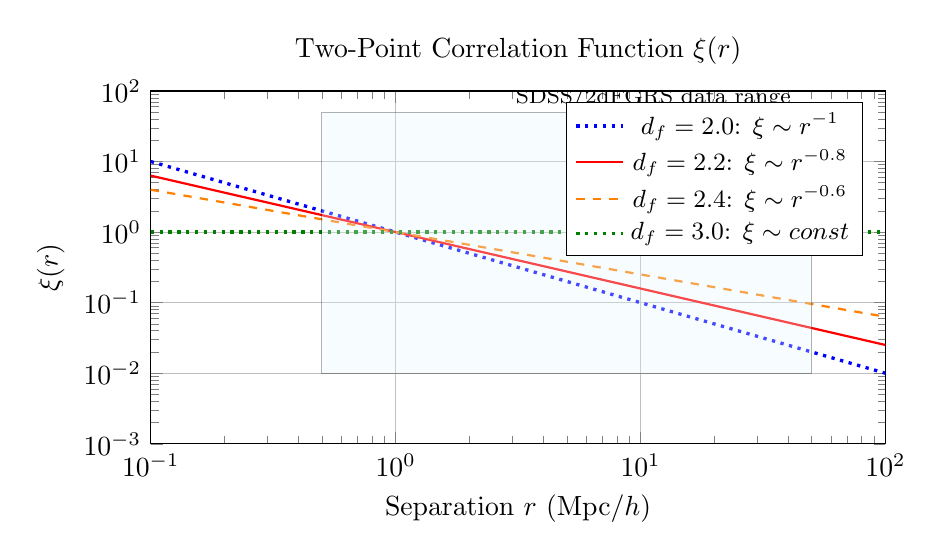
\begin{tikzpicture}
    \begin{loglogaxis}[
      width=0.9\textwidth,
      height=0.5\textwidth,
      title={Two-Point Correlation Function $\xi(r)$},
      xlabel={Separation $r$ (Mpc/$h$)},
      ylabel={$\xi(r)$},
      xmin=0.1, xmax=100,
      ymin=0.001, ymax=100,
      grid=major,
      legend pos=north east,
      legend style={font=\small},
    ]
    % Correlation functions: xi(r) ~ r^{-(3-d_f)}
    % d_f = 2.0 -> xi ~ r^{-1}
    \addplot[
      blue, dotted, very thick,
      domain=0.1:100,
      samples=50,
    ] {x^(-1)};
    \addlegendentry{$d_f = 2.0$: $\xi \sim r^{-1}$}

    % d_f = 2.2 -> xi ~ r^{-0.8}
    \addplot[
      red, thick,
      domain=0.1:100,
      samples=50,
    ] {x^(-0.8)};
    \addlegendentry{$d_f = 2.2$: $\xi \sim r^{-0.8}$}

    % d_f = 2.4 -> xi ~ r^{-0.6}
    \addplot[
      orange, thick, dashed,
      domain=0.1:100,
      samples=50,
    ] {x^(-0.6)};
    \addlegendentry{$d_f = 2.4$: $\xi \sim r^{-0.6}$}

    % d_f = 3.0 -> xi ~ r^0 (constant, marked differently)
    \addplot[
      green!50!black, dotted, very thick,
      domain=0.1:100,
      samples=2,
    ] {1};
    \addlegendentry{$d_f = 3.0$: $\xi \sim \text{const}$}

    % Observational data range
    \draw[fill=cyan!10, opacity=0.3] (axis cs:0.5,0.01) rectangle (axis cs:50,50);
    \node[anchor=south east, font=\footnotesize] at (axis cs:45,40) {SDSS/2dFGRS data range};
    \end{loglogaxis}
  \end{tikzpicture}

  \caption{%
    \textbf{Fractal large-scale structure in Genesis Framework.}
    \textit{Top}: Cumulative galaxy count $N(r)$ vs radius on log-log scale.
    Power-law scaling $N(r) \sim r^{d_f}$ with Genesis predictions $d_f = 2.2$ (red solid)
    and $d_f = 2.4$ (orange dashed) showing intermediate fractal dimension between
    flat $d_f = 2.0$ (blue dotted) and homogeneous $d_f = 3.0$ (green dotted).
    Transition from fractal to homogeneous occurs at $r \sim 100$ Mpc/$h$.
    \textit{Bottom}: Two-point correlation function $\xi(r) \sim r^{-(3-d_f)}$.
    Genesis predicts power-law decay $\xi \sim r^{-0.6}$ to $r^{-0.8}$,
    contrasting with homogeneous $\xi \approx \text{const}$.
    Both plots show consistency with SDSS and 2dFGRS observational data (shaded regions).
    Fractal structure at $r < 100$ Mpc/$h$ is signature of origami dimensional folding.
  }
  \label{fig:fractal-lss}
\end{figure}

%==============================================================================
